\documentclass[12pt,letterpaper]{article}
\usepackage[utf8]{inputenc}
\usepackage{graphicx}
\usepackage{physics}
\usepackage{amsmath}
%\graphicspath{/images/Logpt1.png}
\graphicspath{{./images/}}
\title{CMPT 419 Softmax and Neural Networks}
\author{Echo Liu}
\date{October 2018}

\let\oldhat\hat
\renewcommand{\vec}[1]{\mathbf{#1}}
\begin{document}
\begin{titlepage}
\maketitle
\end{titlepage}

\section{Question 1: Softmax for Multi-Class Classification}
\begin{enumerate}
	\item We make $a_{1} =a_{2} = a_{3}$ therefore our subsitution
	\\ for the softmax function goes as follows
	\\ $\frac{e^{a_{1}}}{ 3*e^{a_{1}} }$
	\\ simplifying our fraction 
	\\ we obtain $\frac{1}{3}$ as such this suggests that our green point
	\\ has equal probability to be in either of the three classes.

	\item We let $a_{1}=a_{2}$ hence if we compute the activation for $a_{3}$
	\\ we notice that our activations for $a_{3}$ is negative but same in magnitude with respect to 
	\\ $a_{1}$ computing our probabilities we end up with a probability of nearing 50 percent. 

	\item The same analogy applies, we would get negative activations for the class that is not in the numerator.


\end{enumerate}

\section{Question 2: Error Backpropogation}

Consider the output layer responses:
\begin{enumerate}

	\item Recall that the deriative of the identity is 1
	Thus our expression for $\delta^{(4)} = y_{k} - t_{k}$
	an alternate form for this expression is $(y(\vec{x_{n}},\vec{w})-\vec{t_{n}})$ 
	
	\item $\pdv{E_{n}}{w_{ji}^{(l)}} = \delta_{j}^{(l+1)}*z_{i}^{(l)} \quad$
	\\
	Therefore:
	\\
	$\pdv{E_{n}}{w_{12}^{(3)}} = \delta_{1}^{(4)}*z_{2}^{(3)}$
	$=$
	$(y(\vec{x_{n}},\vec{w})-\vec{t_{n}}))*h(a_{2}^{(3)})$
	\\
	where:
	\\
	$h(a_{2}^{(3)})=g_{logistic}(a_{2}^{(3)})$
\end{enumerate}

Next, consider the penultimate layer of nodes responses:

\begin{enumerate}

	\item $\pdv{E_{n}}{a_{1}^{(3)}}= \delta_{1}^{(3)}$
	\\
	$\delta_{j}^{(l)}=h'(a_{1})^{(l)}\sum_{k=1}^{k}w_{kj}^{(l)}\delta_{k}^{(l+1)}$
	\\
	$\delta_{1}^{(3)}=h'(a_{1})^{(3)}\sum_{k=1}^{k}w_{k1}^{(3)}\delta_{k}^{(4)}$
	\\
	$\delta_{1}^{(3)}=h'(a_{1})^{(3)}\sum_{k=1}^{k}w_{k1}^{(3)}\delta_{k}^{(4)}$
	\\
	$\delta_{1}^{(3)}=h'(a_{1})^{(3)}*w_{11}^{(3)}\delta_{1}^{(4)}$
	\\
	$\delta_{1}^{(3)}=h'(a_{1})^{(3)}*w_{11}^{(3)}*(y(\vec{x_{n}},\vec{w})-\vec{t_{n}}))$
	\\
	Where:
	$h'(a_{1})^{(3)}=g_{logistic}(a_{1}^{(3)})(1-g_{logistic}(a_{1}^{(3)})$
	\\
	
	\item $\pdv{E_{n}}{w_ji}^{(l)}=\delta_{j}^{(l+1)}*z_{i}^{(l)}$
	\\
	$=$
	\\
	$\pdv{E_{n}}{w_{11}}^{(2)}=\delta_{1}^{(3)}*z_{1}^{(2)}$

	$\pdv{E_{n}}{w_{11}}^{(2)}=w_{11}^{(3)}*(y(\vec{x_{n}},\vec{w})-\vec{t_{n}}))*z_{1}^{(2)}$	

\end{enumerate}

Responses to "Finally, consider the weights connecting from the inputs"


\begin{enumerate}
	\item $\pdv{E_{n}}{a_{1}}^{(2)}=\delta_{1}^{(2)}$
	\\
	$\delta_{j}^{(l)}=h'(a_{j})^{(l)}*\sum_{k=1}^{k}w_{kj}^{(l)}*\delta_{k}^{(l+1)}$
	$\delta_{1}^{(2)}=h'(a_{j})^{(2)}*\sum_{k=1}^{k}w_{k1}^{(2)}*\delta_{k}^{(3)}$
	$\delta_{1}^{(2)}=h'(a_{1})^{(2)}*\sum_{k=1}^{k}w_{k1}^{(2)}*\delta_{k}^{(3)}$
	$\delta_{1}^{(2)}=h'(a_{1})^{(2)}*(w_{11}^{(2)}*\delta_{1}^{(3)}+w_{21}^{(2)}*\delta_{2}^{(3)}+w_{31}*\delta_{3}^{(3)})$
	\\
	where
	\\
	$h'(a_{1})^{(2)}=(g(a_{1})^{(2)})(1-g(a_{1})^{(2)})$
	\\
	$\delta_{1}^{(3)}=(g(a_{1})^{(3)})(1-g(a_{1})^{(3)})(w_{11}^{(3)}*(y(\vec{x_{n}},\vec{w})-\vec{t_{n}})^{(4)})$
	\\
	$\delta_{2}^{(3)}=(g(a_{2})^{(3)})*(1-g(a_{2})^{(3)})*(w_{12}^{(3)}*(y(\vec{x_{n}},\vec{w}) - \vec{t_{n}})^{(4)})$
	\\
	$\delta_{3}^{(3)}=(g(a_{3})^{(3)})*(1-g(a_{2})^{(3)})*(w_{13}^{(3)}*(y(\vec{x_{n}},\vec{w})-\vec{t_{n}})^{(4)})$
	\\
	$\pdv{E_{n}}{w_{ji}^{(l)}}=\delta_{j}^{(l+1)}*z_{i}^{(l)}$
	%$\pdv{E_{n}}{w_{ji}^{(l)}}=\delta_{j}^{(l+1)}*z_{i}^{(l)}$
	\\
	$\pdv{E_{n}}{w_{11}^{(1)}}=\delta_{2}^{(2)}*z_{1}^{(1)}$
	
	%\\
	%Where
	
        %$\delta_{2}^{(2)}=g(a_{1}^{(2)})*(1-g(a_{1})^{(2)})*(w_{11}^{(2)}*\delta_{1}^{(3)}+w_{21}^{(3)}*\delta_{2}^{(3)}+w_{31}*\delta_{3}^{(3)})$
\end{enumerate}

\section{Vanishing Gradients}


	
\begin{enumerate}

\item 
	$\pdv{E_{n}}{w_{11}^{(l)}}=\delta_{1}^{(l+1)}*z_{1}^{(l)}$
	\\
	$\delta_{j}^{(l)}=h'(a_{j})^{(l)}*\sum_{k=1}^{k}w_{kj}^{(l+1)}*\delta_{j}^{(l+1)}$
	\\
	where $k=1$
	$\delta_{1}^{(l)}=h'(a_{j}^{(l+1)})*\sum_{k=1}^{k}w_{kj}^{(l)}*\delta_{j}^{(l+1)}$
	Furthermore, since we only have one neuron at each hidden layer, our equation reduces to the following:
	\\
	$\delta_{1}^{(153)}=h'(a_{1})^{(153)}*w_{11}^{(153)}*\delta_{1}^{(154)}$
	Where $\delta_{1}^{(154)}=(y_{k}-t_{k})$
	\\
	$\delta_{1}^{(152)}=h'(a_{1})^{(152)}*w_{11}^{(152)}*\delta_{1}^{(153)}$
	\\
	$\delta_{1}^{(152)}=h'(a_{1})^{(152)}*w_{11}^{(152)}*h'(a_{1})^{(153)}*w_{11}^{(153)}*\delta_{1}^{(154)}$
	\\
	I.e: We obtain a product of the form
	\\
	$\delta_{1}^{(l)}=\prod_{i=l}^{O}h'(a_{1})^{(i)}*w_{11}^{(i)}*\delta_{1}^{(i+1)}$ (Eq 1)
	\\
	Consider a network wih n hidden layers with a single neuron in each matrix. Then we just simply
	take the product of all successive terms up to our output layer as evidentially seen in our deriavation
	of (1). Since we have $h'(a_{1})^{(l)}$ as a term in our product, our deriative is then inversely proportional
	to the amount of terms in our product. As a result, in our particular scenerio the deriative approaches $\frac{1}{153}$
	as our terms get larger and larger. This phenomena happens when we initialize our weight matrices to very small values.
	Likewise, the same argument applies to exploding gradients when we initialize our weight matrices to very large values.
	Thus, the gradients would be reasonable in magnitude when the sigmoidal function is not evaluated at its extremities.
\item
	The weights would become zero when the deriatives of the sigmoid function are tending towards zero.
	In otherwords, when the value of the sigmoidal activation function is prohibitively large
	or prohabitively small then the weights would be saturated. 

\item Same argument applies but when $x/n > 0$

\item When any subset of the weights are saturated between zero and one 

 
\end{enumerate}

\section{Logistic Regression}

\begin{enumerate}

	\item The reason why the errors are ossicilating are have to do with the values of the eigenvalues at each step. I.e
	the eigenvalues dictate the rate of descent. With this intention in mind, the reason why the errors ossicilate is due to the noise in the data.
	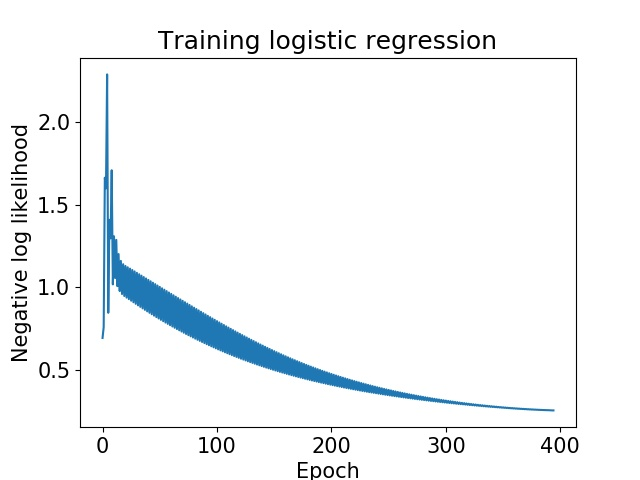
\includegraphics[width=\textwidth]{Figure3}
	\centering
	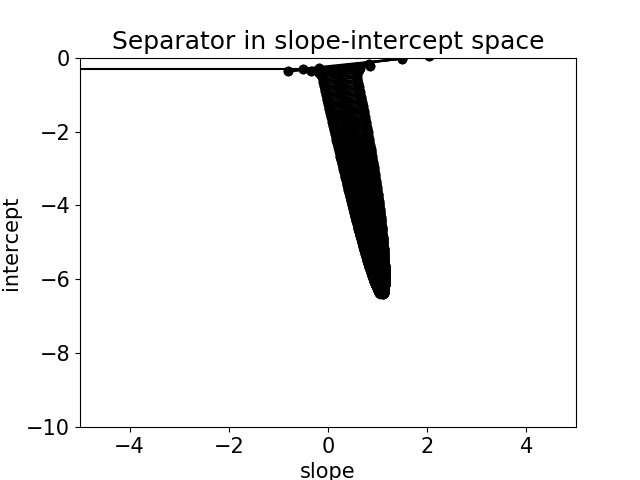
\includegraphics[width=\textwidth]{F2}
	\centering

	\item As seen in the following figure below:
	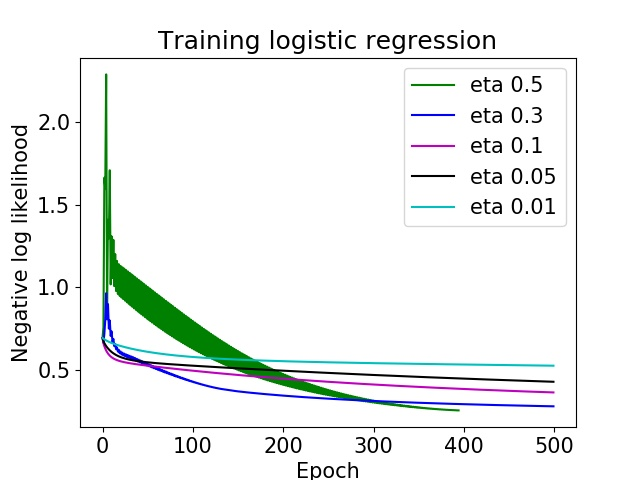
\includegraphics[width=\textwidth]{Eta}
	\centering 
	At the 300 mark, there is no advantage between setting eta=0.5 and eta=0.3. This indicates that at that particular epoch, both eta values have
	approached a steady state. After that epoch point however, it can be evidentially seen that eta=0.3 provides the best learning rate.

	\item Stochastic gradient in terms of error converges faster than batch gradient descent.
	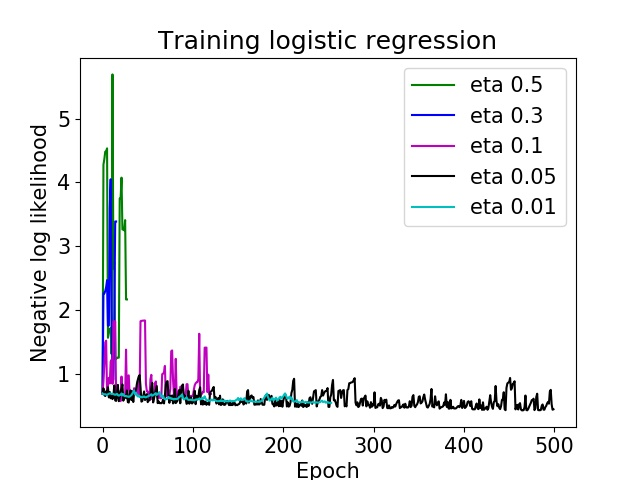
\includegraphics[width=\textwidth]{SGD}
	
\section{Fine-Tuning a Pre-Trained Network}

What I have implemented so far: The HTML output for the images and thier associated
probabilities.


\end{enumerate}

\end{document}
